\section{Classificação e etapas da pesquisa}
\label{natureza}

A elaboração do presente estudo caracterizou-se como uma pesquisa aplicada quanto à sua natureza. Segundo \citeonline{silva2005pesquisa}, a pesquisa aplicada visa gerar conhecimentos para aplicação prática e voltados à solução de problemas específicos e interesses locais.

Do ponto de vista da abordagem do problema a pesquisa classifica-se como qualitativa. Para \citeonline{silva2005pesquisa}, a pesquisa qualitativa preocupa-se com o processo de investigação, sendo que há uma relação dinâmica entre o objeto a ser estudado e o sujeito, estabelecendo-se um vínculo indispensável entre o mundo objetivo e a subjetividade do sujeito. Somada a essa questão, destaca-se que a interpretação dos fenômenos e a atribuição de significados pelo pesquisador é o instrumento-chave da pesquisa qualitativa.

Em relação aos objetivos, a pesquisa é exploratória, pois buscou:

\begin{citacao}
proporcionar maior familiaridade com o problema, com vistas a torná-lo mais explícito ou a constituir hipóteses[...] seu planejamento é, portanto, bastante flexível, de modo que possibilite a consideração dos mais variados aspectos relativos ao fato estudado \cite[p. 41]{gil2002elaborar}.
\end{citacao}

No que concerne aos procedimentos técnicos utilizou-se para o presente estudo: a pesquisa bibliográfica, a documental e o estudo de caso \cite{gil2002elaborar}. Esses procedimentos técnicos referem-se à:

\begin{enumerate}
    \item[a)] Pesquisa bibliográfica: realizada a partir de buscas aos documentos dos principais autores sobre \gls{DSL}: Fowler (2005, 2008) e Voelter (2011, 2013, 2014, 2018). A consulta aos referidos autores possibilitou a identificação de outros materiais sobre a temática, bem como outros pesquisadores utilizados no decorrer do texto. Ademais, utilizou-se a legislação sobre as leis de cotas no sistema de ensino público federal, que foram descritas no Capítulo \ref{chap:historicoversoes};

    
    \item[b)] Pesquisa documental: utilizada durante a análise do histórico do controle de versão do \gls{IFSC}, mediante à busca manual de \textit{commits} e tarefas na ferramenta \texttt{Trello} que continham as palavras-chave ''cotas, sistema de cotas e Departamento de Ingresso (DEING)'' e a posterior identificação dos arquivos relevantes na classificação de candidatos. Nessa análise foram encontrados arquivos contendo as implementações das funcionalidades apresentadas no Capítulo \ref{chap:historicoversoes}, no qual foram detalhadas as linhas de código e as funções envolvidas em 3 (três) versões do sistema de ingresso. Adicionalmente, utilizou-se um \textit{e-mail} (APÊNDICE \ref{chap:apen:emaildeing}), contendo o histórico de demandas sobre o assunto, o qual foi fornecido pelo responsável no setor de ingresso (DEING);
    
    \item[c)] Estudo de caso: Para \citeonline{gil2002elaborar}, o estudo de caso tem o propósito de explorar situações da vida real no contexto do objeto estudado, buscando-se analisar e formular hipóteses sobre a sua aplicação. Por esses motivos foi utilizado nessa pesquisa articulando-se ao estudo de usabilidade da \gls{DSL}, baseado em \citeonline{nielsen2012many}. Para esse autor, quando o público alvo de usuários é variado, normalmente, os testes de usabilidade são realizados em grupos formados de 3 (três) a 4 (quatro) integrantes. Desse modo, considerando os objetivos da presente pesquisa, foram convidadas 20 pessoas com diferentes perfis de experiência, as quais responderam a um exercício proposto para desenvolvimento na \gls{DSL}, bem como a um questionário após a realização dos testes. 
    
\end{enumerate}

    O processo do estudo de caso foi conduzido com base no trabalho de \citeonline{runeson}, o qual define 5 (cinco) passos principais para serem considerados:
    
    \begin{itemize}
        \item[a)] Definir o estudo de caso: objetivos são definidos e o estudo de caso é planejado;
        \item[b)] Preparar a coleta de dados: procedimentos de coleta de dados são definidos;
        \item[c)] Evidenciar a coleta de dados: execução e registro da coleta de dados;
        \item[d)] Analisar os dados coletados;
        \item[e)] Relatar os resultados.
    \end{itemize}

    Considerando a pergunta central da pesquisa, ''Como utilizar uma linguagem de definição de regras do sistema de cotas de modo a melhorar a comunicação entre usuários especialistas e desenvolvedores e, assim, verificar a possibilidade de melhoria no processo de desenvolvimento das regras presentes na legislação?'', foi possível definir as seguintes questões do estudo de caso:
    
    \begin{enumerate}
        \item[a)] É possível a criação de uma linguagem específica de domínio que padronize as definições em comum nas regras de distribuição de vagas?
        
        \item[b)] A utilização da linguagem proposta pode ajudar na produtividade durante o desenvolvimento de alterações na legislação, reduzindo a quantidade de linhas de código a serem implementadas manualmente pelos desenvolvedores?
        
        \item[c)] A definição de regras do sistema de cotas pode ser facilitada com apoio de uma \gls{IDE} que faça validações e forneça recursos específicos para a linguagem proposta?
    \end{enumerate}
    
  
    Para a etapa de preparação da coleta foram apresentados os materiais de apoio elaborados (vídeo explicativo e manual de uso da DSL), e na sequência, o exercício na DSL (APÊNDICE \ref{chap:apen:exercicio}) e o questionário sobre a experiência de uso com os usuários (APÊNDICE \ref{chap:apen:manual}). Esses materiais foram utilizados como instrumentos de coleta de dados com o objetivo de fazer uma avaliação preliminar de uso da DSL Cotas, assim como, de identificar o perfil dos usuários e as principais dificuldades encontradas por eles. O detalhamento do exercício e do questionário serão retomados nas próximas Seções. As evidências da coleta, a análise dos dados coletados e o relato de resultados serão descritos respectivamente nos Capítulos \ref{chap:analise} e \ref{chap:consideracoes}.
 
     A fim de situar o leitor acerca das etapas desenvolvidas na pesquisa, apresenta-se a Figura \ref{fig:etapas}. Nessa Figura, as duas primeiras etapas são responsáveis pelo levantamento conceitual, no qual realizou-se a análise do controle de versão do sistema de ingresso do IFSC e o levantamento dos principais estudos e pesquisas sobre \gls{DSL}s, respectivamente. As etapas seguintes referem-se ao desenvolvimento da DSL Cotas e da API de classificação e aprovação de candidatos. Na sequência, os procedimentos de avaliação e de análise foram compostos pelas etapas de avaliação da API com base no histórico de processos seletivos do IFSC e de aplicação dos instrumentos de coleta com os usuários da DSL Cotas. Com base nesses dados foi possível analisar a viabilidade de melhoria de comunicação entre os usuários de negócio e desenvolvedores a partir da DSL Cotas e, por fim, apresentar os resultados obtidos.
    
    
    \begin{figure}[ht!]
\centering

\caption{\textmd{Etapas da pesquisa}}
\label{fig:etapas}
\fcolorbox{gray}{white}{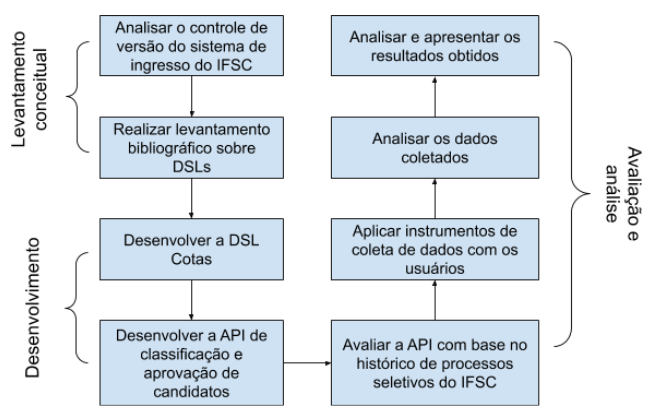
\includegraphics[width=0.76\textwidth]{chapters/metodologia/imagens/etapas.png}}

\par\medskip\textbf{Fonte:} Elaborada pelo autor (2020). \par\medskip

\end{figure}

    
 
    Desse modo, a Seção \ref{ambiente} descreve a metodologia de avaliação da DSL, abordando o perfil dos usuários, o detalhamento do exercício, o questionário aplicado e os critérios utilizados para avaliação da \gls{API}. 
    
    
    
  